\documentclass{article}
\usepackage{xeCJK}
\usepackage{geometry}
\usepackage{amsmath}
\usepackage{graphicx}
\graphicspath{{./images/}}
\geometry{a4paper,scale=0.8}
\begin{document}


\newpage
\section{问题 4}
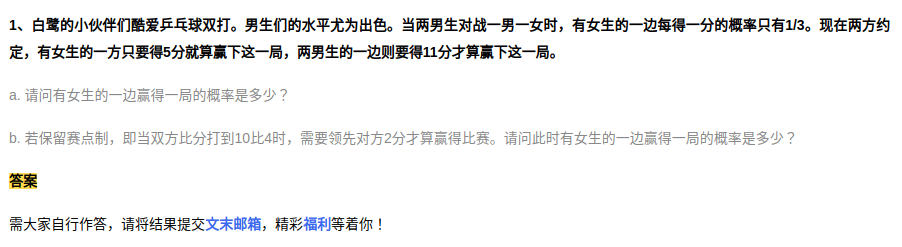
\includegraphics[scale=0.5]{pingpang.png}

a. 考虑女生输的情况的比分有 11:0, 11:1, 11:2, 11:3, 11:4,并且最有一分一定是男生得分。考虑一般情况 11:a的概率为
$$
P(a) = C^a_{10+a} \times (\frac{1}{3})^a \times (\frac{2}{3})^{11}
$$
所以女生输的总概率为
$$
P = \Sigma_{a=1}^{4} P(a) = [C^0_{10} + C^1_{11} \times (\frac{1}{3})^1 + C^2_{12} \times (\frac{1}{3})^2 + C^3_{13} \times (\frac{1}{3})^3 + C^4_{14} \times (\frac{1}{3})^4] \times (\frac{2}{3})^{11} = 0.4040647834709638
$$

所以女生赢一局的概率为 $ 1 - P = 0.5959352165290361 $

\vspace{60pt}

b. 若保留赛点制,前面的计算中,除了11:4的情况外,其他都适合。下面求11:4的情况。
比分为10:4的概率为
$$
P_0 = C^4_{14} \times (\frac{1}{3})^4 \times (\frac{2}{3})^{10}
$$

那么接下来女生要输,可能还要打2个球,4个球,6个球...,并且最后两个球一定是男生连续赢2个。考虑一般情况,再打 a 个球女生输了,a为偶数,那么概率为
$$
P(a) = P_0 \times (\frac{1}{3} \times \frac{2}{3} + \frac{2}{3} \times \frac{1}{3})^{\frac{a-2}{2}} \times (\frac{2}{3})^2 = P_0 \times (\frac{4}{9})^b
$$
其中 $b=\frac{a}{2} = 1,2,3,...$

那么,赛点后女生输的概率为
$$
P_1 = \Sigma^{\infty}_{b=1} P(a) = \Sigma^{\infty}_{b=1}(\frac{4}{9})^b \times P_0 = \frac{4}{5} \times P_0 = 0.17144564390862652
$$

那么女生输的概率为
$$
P = [C^0_{10} + C^1_{11} \times (\frac{1}{3})^1 + C^2_{12} \times (\frac{1}{3})^2 + C^3_{13} \times (\frac{1}{3})^3] \times (\frac{2}{3})^{11} + P_1 = 0.43263905745573483
$$

所以女生赢的概率为 $ 1 - P = 0.5673609425442652 $

\newpage

\section{问题 5}

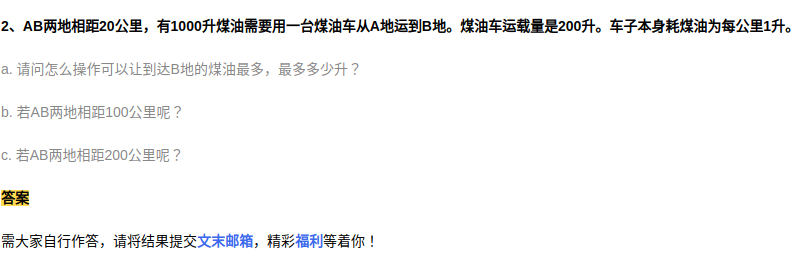
\includegraphics[scale=0.5]{oil.png}

此题就是让车能够移动最少的距离然后把油从A运送到B。考虑AB距离为L,他们的中点为C,如果我们先把油从A运到C,再从C运到B,在这种方案下,A到C的来回次数和原来A到B的来回次数相同。由于在C点的油已经小于在A点的油,所以C到B的来回次数可能要小于原来A到B的来回次数。所以先把所有油运到中点,一定是优于直接从起始点运到末尾。因此,我们把AB这段距离分割的次数越多,油耗就会越小。
设当所有油运到了$x$处,此时总油量为$a$,那么我们运到下一个$x+dx$处,油量变化为$da$
令 
$$ a = 200k+ b $$
即 $ b = a \% 200 $, $k$ 为整数。
则油罐车在这段$ dx $ 上的往返次数为(因为$dx$可以取无限小,所以只要$b > 0$,总可以使得 $b > 2dx$ 成立, 油罐车总要回去把剩余的$b$取来)
$$ 
n = \left\{
    \begin{aligned}
        2k - 1 & , & b = 0 \\
        2k + 1 & , & b > 0 
    \end{aligned}
\right.
$$
所以往前运输 $dx$ 这段距离上的油耗为 $n \times dx$ 所以可以得到每公里油耗$C(a)$为:
$$
C(a) = \frac{da}{dx} = n = 
\left\{
    \begin{aligned}
        9 & , & a \in [1000, 800) \\
        7 & , & a \in [800, 600) \\ 
        5 & , & a \in [600, 400) \\
        3 & , & a \in [400, 200) \\
        1 & , & a \in [200, 0) \\
    \end{aligned}
\right.
$$

所以可以求得问题中的解:


当 AB 距离 20km 时候,油耗 = 9L/km, 所以到达 B 处时候最大油量为 $1000 - 9 \times 20 = 820$

当 AB 距离为 100km 时候, 到达B 处的最大油量为
$$ 
400 - (100 - (\frac{200}{9} + \frac{200}{7} + \frac{200}{5})) \times 3 = 372.3809523809524
$$


当 AB 距离为 200km的时候,到达B 处的最大油量为
$$
200 - (200 - (\frac{200}{9} + \frac{200}{7} + \frac{200}{5} + \frac{200}{3})) \times 1 = 157.46031746031747
$$

\newpage
\section{问题6}
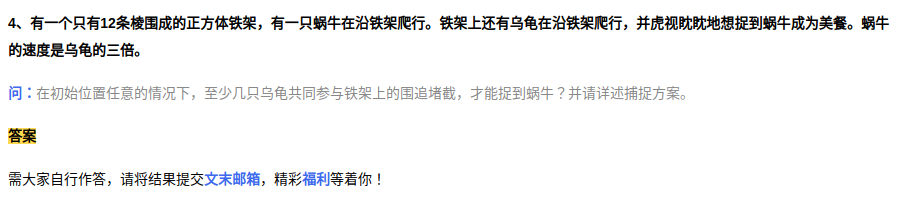
\includegraphics[scale=0.5]{turtle.png}

最少需要 3 只乌龟。首先 1 只乌龟显然追不上。2 只乌龟时候,只要蜗牛一直保持不跟那两只乌龟在同一个面上就不会被抓到。下面给出 3 只乌龟一定能抓到的策略:

3 只乌龟先不管蜗牛的位置,直接走到图中 A, B, C 三个点。此时,蜗牛有三种情况:(1)在D点、(2)在E点(于F、G两点等效), (3)在DE中间

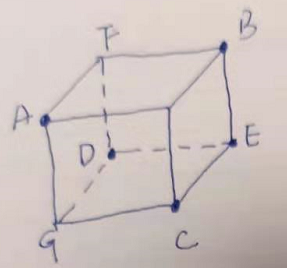
\includegraphics[scale=0.5]{cube01.png}

\vspace{60pt}

现在分别讨论这三种情况

情况1: 乌龟在A、B、C三点,蜗牛在D点。此时,三只乌龟运动方向如图箭头所示。当三只乌龟分别走了$\frac{1}{3}$ 棱长的时候,此时如果蜗牛运动到了E点(其他两点等效),那么B乌龟要观察蜗牛的下一步运动,如果蜗牛要往B点走,那么B乌龟就要掉头返回也往B走。因为蜗牛速度是乌龟3倍,所以蜗牛最快也只能和B乌龟相遇在B点被捕捉。如果蜗牛不往B走了,B蜗牛就继续望F走。否则就继续往前走。按照这个策略一直走,三只乌龟最终会在G、F、E点,而蜗牛就被困在了D、E之间。最终会被抓到。

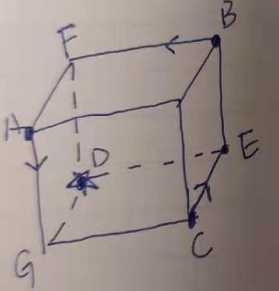
\includegraphics[scale=0.5]{cube02.png}

\vspace{60pt}

情况2: 乌龟在A、B、C三点,蜗牛在E点。A 乌龟想G点移动,而B、C乌龟观察E点处蜗牛的运动。若蜗牛从E点往D点走,则B蜗牛往F走,C蜗牛网E走。这样走下去,最终会到情况1中的状态而被捕获。若E处蜗牛中途返回E,则B、C乌龟也分别返回。当A蜗牛到达G点时候,若蜗牛在E点,则其他两只乌龟在B、C点,此时乌龟观察E点的蜗牛的运动,若E不动,则G点乌龟往D走,若E向D走,则B->F,C->E,G点乌龟不动。这样最终也会达到情况1中的 状态而被捕获。

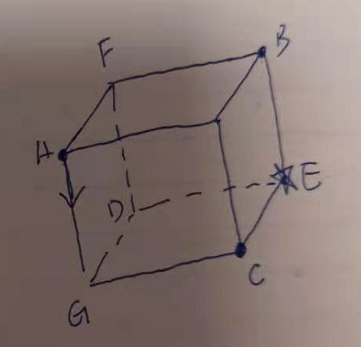
\includegraphics[scale=0.5]{cube03.png}

\vspace{60pt}

情况3: 乌龟在A、B、C三点,蜗牛在D、E中间。前面两种情况,蜗牛在D点和E点都必然被捕获,在中间最后总会落到情况1、2中的一种。所以必然也会被捕获。

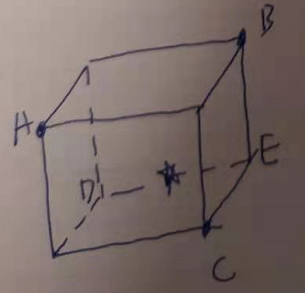
\includegraphics[scale=0.5]{cube04.png}

由此,最少需要 3 只乌龟就可以捉住蜗牛。



\newpage
\section{问题 7}
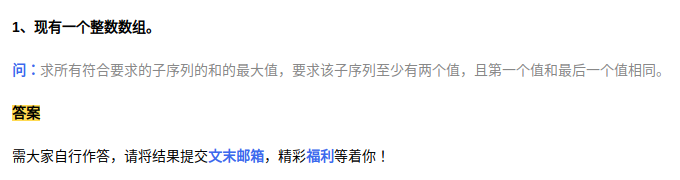
\includegraphics[scale=0.7]{algo.png}
因为我是做IT的,做的算法题比较多。对于这个题目,有两点可以改进。第一,算法题要给出数据范围。比如这个数组多大?数组中每个数多大?因为数据范围直接决定了需要采取的算法。第二,需要说明子序列的定义。在计算机算法这边,子序列是指给定一个序列,删掉任意个元素后得到的序列。我就按照这个定义来做这个题目。



\end{document}